\section{Вычислительные эксперименты}

    \subsection{Алгоритм}
        Для компьютерного вычисления будем использовать метод Рунге-Кутты, с помощью которого получим численное решение системы дифференциальных уравнений с заданными параметрами. После чего построим графики решений на координатной и фазовой плоскостях.


    \subsection{Программа}
        Для расчётов и визуализации был использован язык Python с библиотеками numpy и matplotlib.

        \lstinputlisting[language=Python,
        captionpos=t,
        style=colored,
        basicstyle=\footnotesize\dejavu,
        frame=lines]{src/2model.py}

    \subsection{Результаты}
        Построим несколько решений системы с одинаковыми параметрами, но разными начальными условиями, в том числе и точку равновесия.

        \subsubsection{Эксперимент 1}
        Возьмём параметры $a = 2, c = 0.5, b = 1, d = 0.5$ и покажем графически результаты.

        \begin{figure}[H]
            \centering
            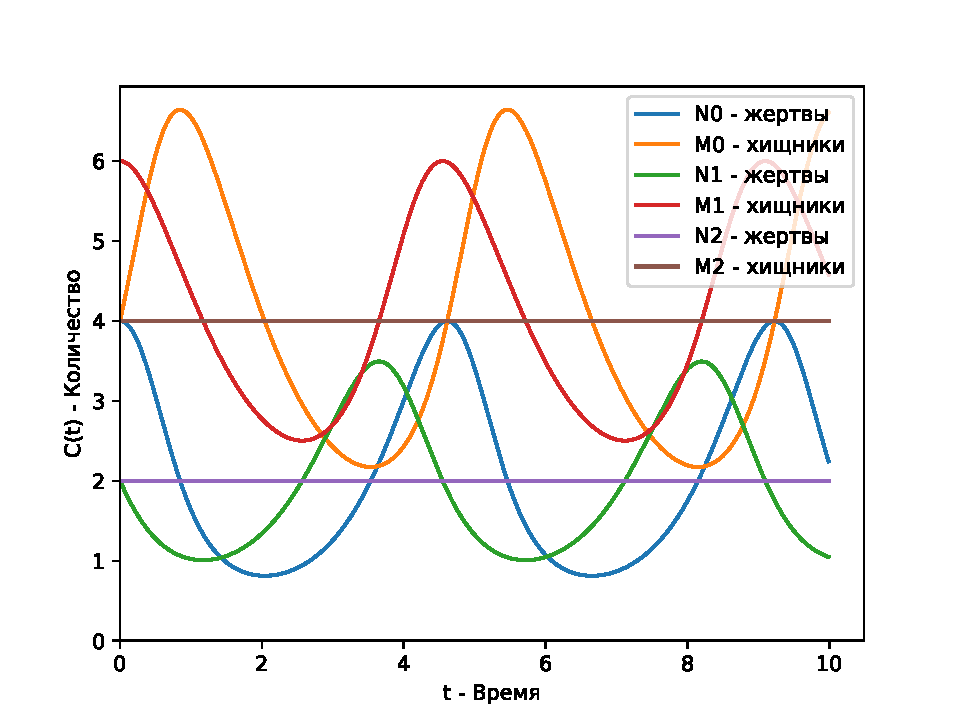
\includegraphics[width=15cm]{pictures/population.pdf} 
            \caption{Решения с начальными условиями $x_0=(4,4), ~ x_1 = (2,6), ~ x_2 = (N_e, M_e)$}\label{exp1t}
        \end{figure}
        Как можем увидеть (Рис. \ref{exp1t}), объёмы популяций изменяются с некоторым периодом. Эти популяции взаимодействуют таким образом, который мы описывали при построении модели. Также заметим, что объём популяций, заданный точкой равновесия $ x_2 $, не изменяется.


        Теперь построим решения на фазовой плоскости $ (N, M) $.
        \begin{figure}[H]
            \centering
            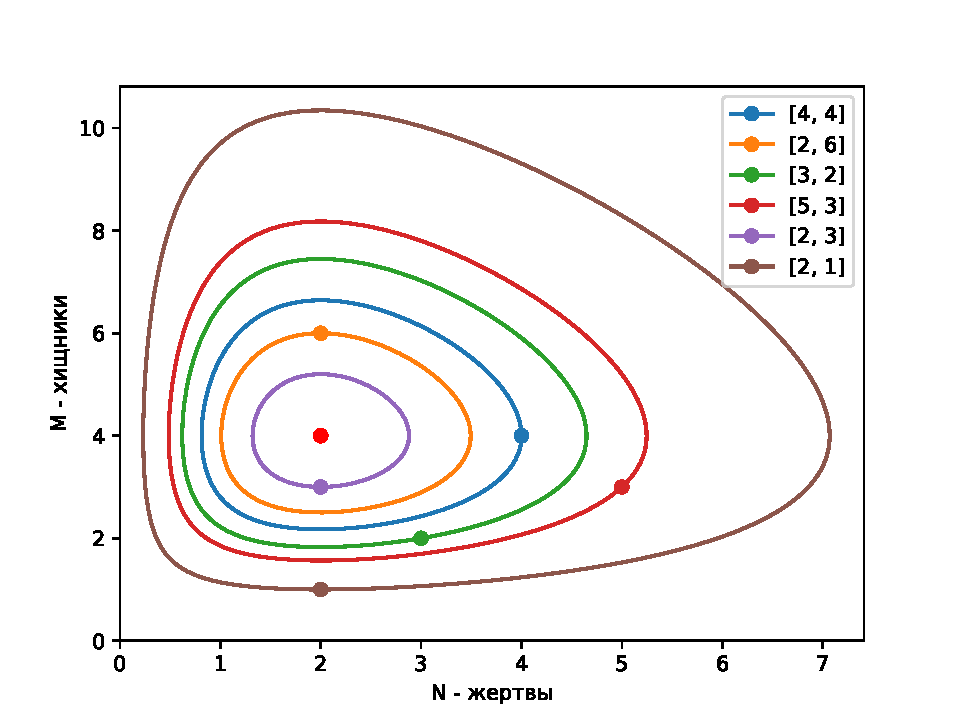
\includegraphics[width=15cm]{pictures/population3.pdf}
            \caption{Решения с указанными начальными условиями на интервале времени $ [0, 10] $.}\label{exp1p}
        \end{figure}
        Точками на рисунке \ref{exp1p} указаны начальные условия, а центральная красная точка -- положение равновесия.
        При анализе мы выяснили, что точка равновесия является неасимптотически устойчивой, из-за чего мы можем видеть циклы на фазовой плоскости. Это также описывается соотношением переменных из первого интеграла системы уравнений.

        Однако, мы построили на таком интервале времени, когда все циклы замкнулись. Уменьшим интервал. 


        \begin{figure}[H]
            \centering
            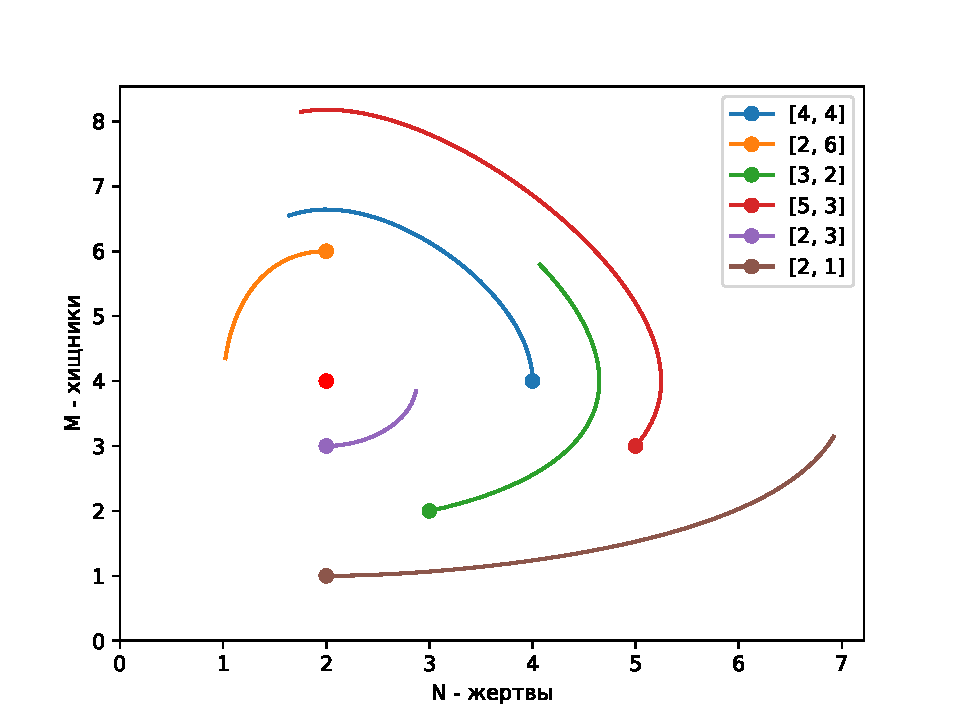
\includegraphics[width=12cm]{pictures/population4.pdf}
            \caption{Решения с указанными начальными условиями на интервале времени $ [0, 1] $.}\label{exp1p2}
        \end{figure}
        На рисунке \ref{exp1p2} на меньшем интервале времени все циклы остались незамкнуты и мы можем увидеть, что они изменяются по направлению против часовой стрелки на данной фазовой плоскости.

        На данном примере мы отчётливо увидели действие ненулевой точки равновесия на систему. Подберём такие параметры, чтобы увидеть действие нулевой точки равновесия.


        \subsubsection{Эксперимент 2}
        Возьмём параметры $a = 2, c = 2, b = 1, d = 4$.
        \begin{figure}[H]
            \centering
            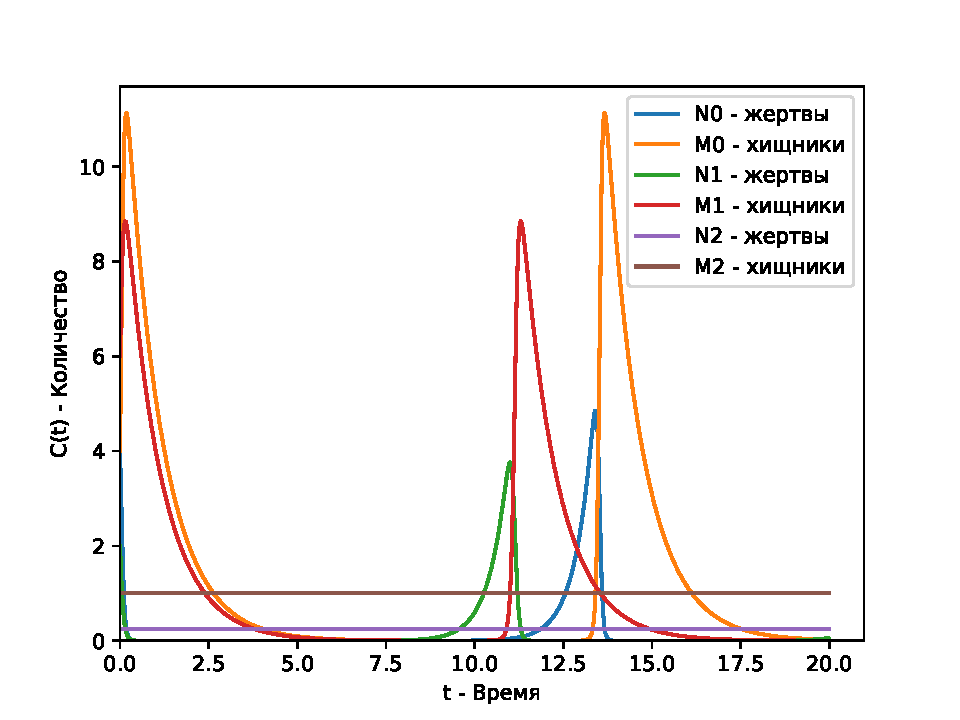
\includegraphics[width=15cm]{pictures/population2.pdf}
            \caption{Решения с начальными условиями $x_0=(4,4), ~ x_1 = (2,6), ~ x_2 = (N_e, M_e)$}\label{exp2t}
        \end{figure}
        Как можно увидеть (Рис. \ref{exp2t}), реализация модели с данными параметрами получилась более <<резкой>>. Уменьшение популяции жертв и увеличение популяции хищников происходит намного быстрее, по сравнению с предыдущим экспериментом.

        Обе популяции сильно приближаются к вымиранию. Небольшая погрешность в вычислениях или какое-либо внешнее взаимодействие реальном мире может довести популяцию до полного вымирания.

        \begin{figure}[H]
            \centering
            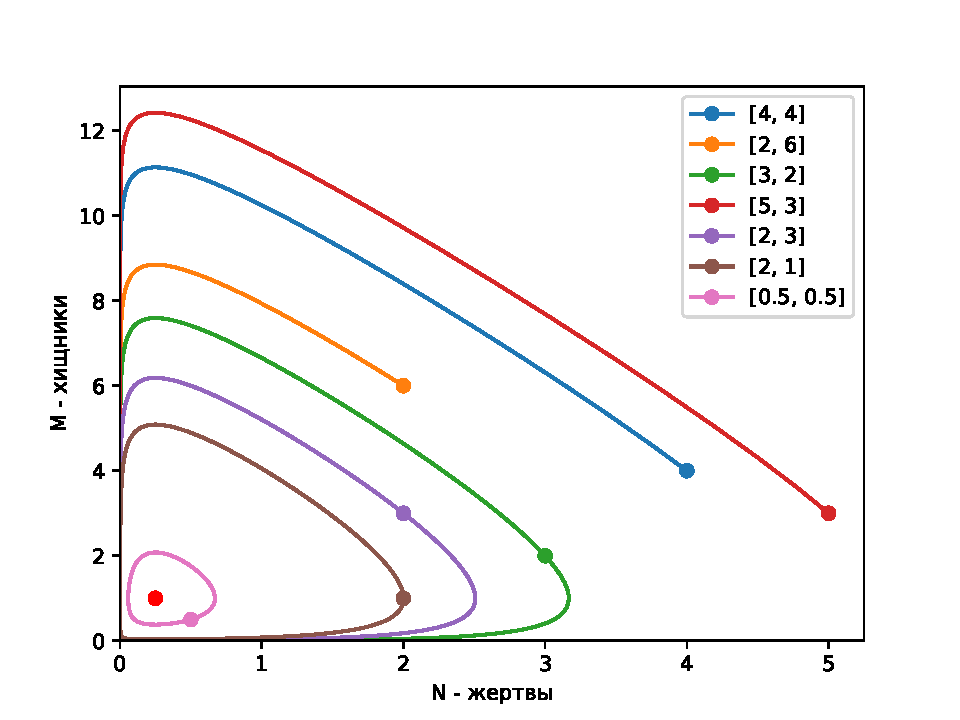
\includegraphics[width=15cm]{pictures/population5.pdf}
            \caption{Решения с указанными начальными условиями на интервале времени $ [0, 10] $.}\label{exp2p}
        \end{figure}
        На фазовой плоскости (Рис. \ref{exp2p}) на данном интервале времени замкнулись не все циклы. Это связано с тем, что популяции уменьшаются до очень маленьких значений, <<выбраться>> из которых займёт больший промежуток времени. Но в этот раз можем увидеть действие нулевой точки равновесия -- седла. Поскольку движение на плоскости происходит против часовой стрелки, то по оси $ M $, как и было получено при анализе $(\lambda_2 < 0)$, движение происходит к началу координат, никогда не пересекая ось $ M $. Аналогично движение по оси $N$ будет происходить, но от начала координат $(\lambda_1 > 0)$. 


